% This is samplepaper.tex, a sample chapter demonstrating the
% LLNCS macro package for Springer Computer Science proceedings;
% Version 2.21 of 2022/01/12
%
\documentclass{llncs}
%
\usepackage[T1]{fontenc}
\usepackage{float}
\usepackage{graphicx}
\usepackage[english]{babel}
\usepackage{booktabs}
\usepackage{url}
\usepackage{hyperref}
\usepackage{listings}
\usepackage{color}
\renewcommand{\floatpagefraction}{0.8}
\renewcommand\UrlFont{\color{blue}\rmfamily}
\urlstyle{rm}
\definecolor{dkgreen}{rgb}{0,0.6,0}
\definecolor{gray}{rgb}{0.5,0.5,0.5}
\definecolor{mauve}{rgb}{0.58,0,0.82}

\lstset{frame=tb,
  language=C++,
  aboveskip=3mm,
  belowskip=3mm,
  showstringspaces=false,
  columns=flexible,
  basicstyle={\small\ttfamily},
  numbers=none,
  numberstyle=\tiny\color{gray},
  keywordstyle=\color{blue},
  commentstyle=\color{dkgreen},
  stringstyle=\color{mauve},
  breaklines=true,
  breakatwhitespace=true,
  tabsize=3
}
\begin{document}
%
\title{The Knapsack Problem}
%
\author{Andrei RUSĂNESCU,
Gabriel-Ioan PAVEL,
Amir FALLAH-MIRZAEI,
323CC}
%
\institute{University Politehnica of Bucharest}
%
\maketitle
%
\begin{center}
	\href{https://github.com/andreirusanescu/Algorithm-Analysis-Knapsack-Problem}{Click here for GitHub repository}
\end{center}
\begin{abstract}
The present paper analyses several algorithms that solve the Knapsack problem,
taking into account both the speed and the memory used by the program. It
presents three solutions, two of which always generate the correct answer, and
one that obtains a result close to the right one.

\end{abstract}
%
%
\section{Introduction}
The Knapsack problem derives its name from the situation faced by someone who wants
to fill their limited-capacity knapsack with the most valuable items that can fit.
You can choose whether to put it in the bag or not put it at all, hence the name
"0/1 Knapsack Problem". The problem has been studied for more than a century, with
writings dating as far back as 1897. 

\section{Practical Applications}
The Knapsack Problem and its variations have a multitude of real life applications
including financial modeling, production and inventory management systems, stratified
sampling, design of queuing network models in manufacturing, and control of traffic
overload in telecommunication systems.

\subsection*{1. Financial Modeling}
\begin{itemize}
    \item \textbf{Investment Portfolio Selection}: In finance, the Knapsack Problem
        is used to select a combination of investment assets that maximize returns while
        staying within a budget or risk tolerance. This involves balancing the trade-offs
        between different financial instruments like stocks, bonds, and derivatives.
    \item \textbf{Capital Budgeting}: Companies use this problem to decide how to
        allocate limited capital resources among various potential projects to maximize returns.
\end{itemize}

\subsection*{2. Production and Inventory Management Systems}
\begin{itemize}
    \item \textbf{Optimal Resource Allocation}: In production, the problem helps in
        determining the best way to allocate limited resources like raw materials or machinery
        to different products to maximize output or profit.
    \item \textbf{Inventory Control}: It is applied to decide which items to stock in
        limited warehouse space, ensuring maximum profitability or utility while minimizing costs.
\end{itemize}

\subsection*{3. Stratified Sampling}
\begin{itemize}
    \item \textbf{Survey Design}: In statistics, the Knapsack Problem helps in stratified
        sampling by selecting a sample that represents different strata or subgroups of a population
        in a cost-effective way, ensuring that the sample is both diverse and within budget constraints.
\end{itemize}

\subsection*{4. Design of Queuing Network Models in Manufacturing}
\begin{itemize}
    \item \textbf{Production Line Optimization}: In manufacturing, the problem aids in the design
        and optimization of queuing networks, where the goal is to minimize waiting times and costs
        while maximizing throughput. This involves selecting the right combination of machines, processes
        and workflows within budgetary and space constraints.
\end{itemize}

\subsection*{5. Control of Traffic Overload in Telecommunication Systems}
\begin{itemize}
    \item \textbf{Bandwidth Allocation}: The Knapsack Problem is used to allocate limited bandwidth
        resources to various communication channels or services to maximize overall network efficiency
        and quality of service.
    \item \textbf{Data Packet Prioritization}: It helps in determining which data packets should
        be transmitted first based on their priority and the available network capacity to prevent
        congestion and optimize network performance.
\end{itemize}

\section{NP-Complete Proof}
\paragraph{General overview}
The Knapsack problem has as inputs: \textbf{W} - the maximum weight of the sack, \textbf{N} - the number of objects and the \textbf{Objects} themselves that have as proprieties: \textbf{weight and profit}. The program returns the maximum profit that you can get without exceeding the weight limit\textit{(this format is used everywhere else in the paper)}. But, as to respect the algorithms' return convention we modify it so, the knapsack function also takes as input \textbf{P} - the profit goal and now returns \textit{true} if the goal was met, or \textit{false} otherwise.  

\[
 Knapsack \in NP-Complete \Rightarrow Knapsack \in NP,\ Knapsack \in NP-Hard
\]
\subsection{NP Proof}
We show that the problem can be solved using a nondeterministic algorithm in \textit{NP time} and a solution can be checked in \textit{P time}.


\begin{lstlisting}[language=Python] 
def knapsack(W, N, P, Objects):
    seen = N * [0]
    current_weight = 0
    current_profit = 0
    sack = []

    # generation phase
    for i = 1 : N:
        c = choice(0...N)
        if c != 0:
            if seen[c] == 1:
                fail()
            seen[c] = 1
            sack.append(Objects[c])
            current_weight += Objects[c]['weight']
            if current_weight > W:
                fail()
            current_profit += Objects[c]['profit']

    # testing phase
    if current_profit == P:
        success()

    fail()
\end{lstlisting}

\subsection{NP-Hard Proof}
We assume to be known that the \textbf{SubsetSum problem} is included in the NP-Hard class. So we seek to prove that SubsetSum problem reduces polynomially to the Knapsack problem.
\[
Subset Sum \leq_{P} Knapsack \Rightarrow Knapsack \in NP-Hard
\]
SubsetSum takes as input: \textbf{M} - an array of integers and \textbf{Sum} - the target sum. It outputs \textit{true} if there is a subset of numbers from the array that has the sum equal to \textit{Sum}, or \textit{false} otherwise.
The transfer function can be computed in \textbf{polynomial time} and it is as follows:

\[SubsetSum(M, Sum) \rightarrow Knapsack(W, N, P, Objects)\]
\[W = Sum, \ N = len(M), \ P = Sum, \ Objects = \{(x_i,x_i)\ |\ x_i \in M \} \]
\textit{Correctness proof $(\Leftrightarrow)$} If $SubsetSum(M, Sum) = true \Leftrightarrow \exists S\in M$ so that the sum of S is equal to $Sum = W = P$ $\Leftrightarrow S' = \{(x_i, x_i) | x_i \in S\} \subseteq Objects \Leftrightarrow S'$ is a solution of the Knapsack problem $\Leftrightarrow Knapsack(W, N, P, Objects) = true$.


\subsection{Proof Conclusion}
Having demonstrated that \textbf{Knapsack} is of class NP and of class NP-Hard we can finally say that it is also a member of the NP-Complete class.


\section{Description of the algorithms}
\subsection{Dynamic programming}
There are two approaches to solve this problem using dynamic programming:
using a memoization table (top-down) or tabulation (bottom-up). 
\begin{itemize}
    \item \textbf{Memoization}: Using recursion to solve the Knapsack Problem results in an exponential
        time complexity. This is due to the fact that the algorithm recomputes functions that have already
        been processed multiple times. Instead of recomputing these values, we can utilize a \textit{memoization}
        table to store the results of these functions. By doing so, we can significantly reduce the time complexity and make the algorithm more efficient. Memoization involves storing the results of previously computed subproblems in a table (often a two-dimensional array).
    \item \textbf{Tabulation}: This is the approach I chose to implement in code, because it is usually
        faster then the memoization one owing to its iterative nature. Despite calculating all the
        combinations of objects in the knapsack, the tabulation method is known as "Bottom-Up" since
        it builds the solution incrementally from the smallest subproblems to the overall problem.
        Tabulation involves filling up a table (typically a two-dimensional array, even though it can be
        done using a one-dimensional array). Each entry in the table represents the solution to a subproblem,
        and the solution to the overall problem is derived from these subproblem solutions.
\end{itemize}

\begin{lstlisting}
int N, G; // N - the number of objects, G - the capacity of the knapsack
std::vector<std::vector<int>> dp; // dp matrix
std::vector<int> weights, values; // weights and values of the objects
inline int knapsack() {
        for (int i = 0; i <= N; ++i)
                dp[i][0] = 0;
        for (int j = 0; j <= G; ++j)
                dp[0][j] = 0;

        for (int i = 1; i <= N; ++i) {
                for (int w = 1; w <= G; ++w) {
                        if (weights[i - 1] <= w)
                                dp[i][w] = std::max(values[i - 1] + dp[i - 1][w - weights[i - 1]], dp[i - 1][w]);
                        else
                                dp[i][w] = dp[i - 1][w];
                }
        }
        return dp[N][G];
}

inline std::vector<int> find_objects() {
        std::vector<int> res;
        int m = N, n = G;
        while (n > 0 && m > 0) {
                if (dp[m][n] != dp[m - 1][n]) {
                        n -= weights[m - 1];
                        res.push_back(m);
                }
                --m;
        }
        std::reverse(res.begin(), res.end());
        return res;
}
\end{lstlisting}

To begin with, the code is as fast as it can possibly be, while still being intelligible. I used inlining
to suggest the compiler to paste this code where it is called from in order to reduce the potential overhead
of pushing registers onto the stack. Furthermore, I used global variables that are initialized in the main
procedure, due to the fact that these two functions are benchmarked using the Google Benchmark for C++. I
wanted to make a separation between I/O (filling the data), allocations and initializations, and the true
computing effort these functions bring.

Each row in the matrix corresponds to an object, while each column represents a maximum weight capacity.
The entry dp[i][w] denotes the maximum profit achievable using the first \textbf{i} objects with a weight
limit of \textbf{w}. This value is determined by taking the maximum between two options: the sum of the
current object's profit and the optimal profit from the remaining capacity, and the best profit obtained
without including the current object. In essence, it captures the overall maximum profit for the given weight
constraint, the last cell being the result. The function responsible for finding the objects that were put
in the bag is doing reverse engineering on the matrix. If the profit obtained for the current row is different
than the one above it, meaning the current object was used, so it is selected, otherwise, the current value
is originating from an upper row.


\subsubsection{Complexity Analysis}
\paragraph{Time Complexity}
The algorithm involves nested loops to fill the dynamic programming (DP) table:
The outer loop runs from 1 to \textit{N} (the number of objects), resulting in \textit{N} iterations.
The inner loop runs from 1 to \textit{G} (the capacity of the knapsack), resulting in \textit{G} 
iterations. For each combination of \textit{i} (object) and \textit{w} (weight), a constant amount
of work is done, either updating the DP table or performing a comparison. Thus, the overall time
complexity of the algorithm is $\mathcal{O}(N*G)$.

\paragraph{Space Complexity}
The space complexity is determined by the DP table, which is a two-dimensional vector of size 
\textit{(N+1)*(G+1)}. This results in a space complexity of $\mathcal{O}(N*G)$.
Additionally, the \textit{find objects} function uses a vector to store the selected objects, which 
in the worst case, may require space proportional to N, but this does not change the overall space 
complexity.

\subsubsection{Advantages and Disadvantages}
\paragraph{Advantages}
The main advantages are the speed of execution, as the result can be obtained in a reasonable amount
of time, and the avoidance of issues that might arise with recursion, such as stack overflow.

\paragraph{Disadvantages}
The main disadvantages include the large memory usage due to the DP table and the fact that the 
matrix size cannot be dynamically adjusted without recalculating the values.

\subsection{Backtracking}

This approach explores every possible combination of objects recursively. The algorithm is initiated
by the main procedure, which sets up the necessary variables and calls the main backtracking
function. In this context, \textbf{G} represents the maximum weight the knapsack can carry, 
\textbf{maxx} is the maximum profit found so far. The process concludes by returning the best 
possible result. The selection of the indexes is done when a subset of N elements has been explored
and its profit is the current maximal value.


\begin{lstlisting}
int N, G;
int maxx;
std::vector<int> weights, values;
std::vector<int> selection, current_selection;

int knapsack(int index, int curr_weight, int curr_profit) {
        if (index == N) {
                if (curr_profit > maxx) {
                        maxx = curr_profit;
                        selection = current_selection;
                }
                return maxx;
        }

        if (curr_weight + weights[index] <= G) {
                current_selection.push_back(index + 1);
                maxx = std::max(maxx, knapsack(index + 1, curr_weight + weights[index], curr_profit + values[index]));
                current_selection.pop_back();
        }
        return std::max(maxx, knapsack(index + 1, curr_weight, curr_profit));
}
\end{lstlisting}

For each function call, the algorithm checks if the current object can be added without exceeding 
the maximum weight. If it can, the function updates the current maximum profit and continues to 
explore deeper. If not, it skips adding the object. The recursion stops when all combinations of
objects have been considered.

The function iterates over all objects starting from a given \textbf{index}. For each object, it 
adds its weight and value to the current totals, then dives deeper into the recursion. After 
exploring that path, it removes the object's weight and value to backtrack and explore other 
possibilities.

\subsubsection{Complexity Analysis}
\paragraph{Time Complexity}
The main factor contributing to the time complexity is the exhaustive nature of the algorithm, it 
explores every possible subset of objects. This results in \( 2^n \) iterations, as each object can 
either be included or excluded. Therefore, the time complexity is $\mathcal{O}(2^n)$, which grows
exponentially with the number of objects.

\paragraph{Space Complexity}
The space complexity is driven by the depth of the recursion stack. With n objects to check, the 
stack's depth can reach up to \textit{n}, making the space complexity $\mathcal{O}(n)$.

\subsubsection{Advantages and Disadvantages}
\paragraph{Advantages}
One of the main advantages of the backtracking approach is its simplicity. The algorithm is
straightforward to implement and understand, making it an excellent choice for educational purposes
or scenarios where optimality is required for small inputs. Additionally, it doesn't require 
significant memory beyond the recursion stack and a few auxiliary variables.

\paragraph{Disadvantages}
The primary drawback is the method's inefficiency due to its brute-force nature. The exponential 
time complexity makes it impractical for large input sizes, as it results in a vast number of
redundant calculations. This inefficiency becomes a major limitation, especially when compared to
more optimized approaches like dynamic programming.


\subsection{Greedy}

To solve the problem using an algorithm that provides a result close to the correct one I used a
greedy approach. It solves the fractional knapsack problem. The algorithm uses a heuristic based on
the value-to-weight ratio of items to make decisions. Basically, it sorts the objects based on the
value to weight ratio and then fills the bag with the objects until the last one that is divided.
If the sorting of the objects somehow is the correct order, the objects are not truncated at all.
The overall value is close to the correct one based on a large number of tests.

\begin{lstlisting}
int N, G;
std::vector<std::vector<int>> pairs;
std::vector<int> selection;

struct fcmp {
    bool operator()(const std::vector<int> &a, const std::vector<int> &b) {
        double r1 = (double)a[1] / (double)a[0];
        double r2 = (double)b[1] / (double)b[0];
        return r1 > r2;
    }
};

double knapsack() {
    std::sort(pairs.begin(), pairs.end(), fcmp());
    int current_weight = G;
    double res = 0;
    for (int i = 0; i < N; ++i) {
        if (pairs[i][0] <= current_weight) {
            current_weight -= pairs[i][0];
            selection.push_back(pairs[i][2]);
            res += pairs[i][1];
        } else {
            selection.push_back(pairs[i][2]);
            res += pairs[i][1] * ((double)current_weight) / (double)pairs[i][0];
            break;
        }
    }

    return res;
}
\end{lstlisting}

I used a vector of objects that have 3 values, the weight, the value and the corresponding index.
For sorting, I used struct fcmp to provide a sorting logic for the sort() function.


\subsubsection{Complexity Analysis}
\paragraph{Time Complexity}
The time complexity of the algorithm is $\mathcal{O}(NlogN)$ due to the sorting step, where $N$ is
the number of items. After sorting, the algorithm iterates through the list of items, which takes $\mathcal{O}(N)$.
time. Thus, the overall time complexity is dominated by the sorting step, resulting in 
$\mathcal{O}(NlogN)$.

\paragraph{Space Complexity}
The space complexity is $\mathcal{O}(N)$ because the algorithm uses additional space to store the
list of items and the selection vector.

\subsubsection{Advantages and Disadvantages}
\paragraph{Advantages}
The algorithm is efficient and easy to implement, with a relatively low time complexity of 
$\mathcal{O}(NlogN)$. It provides a quick approximation for the knapsack problem, especially useful
when an exact solution is computationally expensive. The greedy approach ensures that the solution
is close to optimal for the fractional knapsack problem.

\paragraph{Disadvantages}
The algorithm may not provide the exact optimal solution for the 0/1 knapsack problem, where items
cannot be divided. It relies on a heuristic (\textit{value-to-weight} ratio) that may not always
yield the best solution for specific instances of the problem. The solution's accuracy depends on 
the distribution of item weights and values; in cases where high-value items have low weight, the 
algorithm performs well, but it may underperform in other cases.

\section{Testing and Evaluation}
The tests are 30 in number and were partly generated using a python script that generated tests with
sizes between 20 and 100 and weights randomly chosen between 500 and 1000. The other part is made of
4 tests I chose from an online resource I cited in the bibliography. To run the benchmark, you should
execute the $run\_benchmarks.sh$ script and it will write the results in the 
tests/benchmarks folder.

For the benchmark test I used my personal laptop with an AMD Ryzen 7 3750H with Radeon Vega Mobile
Gfx 2.30 GHz, 16.0 GB of RAM (13.9 GB usable), running Ubuntu 22.04. The tests where run using the
gcc compiler, version gcc version 11.4.0 with the flags: -std=c++11 -isystem utils/benchmark/include 
-L../utils/benchmark/build/src -lbenchmark -lpthread. All the tests where run with the laptop plugged
in, on the Turbo mode from Ubuntu.

The results are summarized in the tables below, presenting the performance of each algorithm. The 
number of \textit{iterations} for each benchmark test is determined automatically by the 
benchmarking tool, which ensures that the functions are called a sufficient number of times to 
provide reliable measurements. Each line corresponds to a test. The tests are located in the tests/input folder.

\subsection{Performance Analysis}
1. \textbf{Greedy} Algorithm:
Speed: The Greedy algorithm consistently outperforms the other two in terms of speed. This
efficiency is due to its simplistic approach, which just sorts the items and then fills the bag.
Complexity: The Greedy algorithm operates with a time complexity of $\mathcal{O}(NlogN)$. However, it does not guarantee the optimal solution for the problem.
Use Case: Best suited for scenarios where speed is crucial, and the problem constraints or inputs 
naturally lend themselves to a near-optimal solution, close to the correct one.
\newline
2. \textbf{Dynamic Programming} (DP):
Speed: The DP approach shows moderate performance, sitting between the Greedy and Backtracking 
methods. This is expected given its polynomial time complexity.
Complexity: With a time complexity of $\mathcal{O}(N*W)$,  where N is the number of items and 
W is the maximum weight capacity, DP provides a balance between optimality and efficiency. It 
ensures the optimal solution by considering all possible combinations of items up to the maximum
weight.
Use Case: Ideal for scenarios where an exact solution is necessary.
\newline
3. \textbf{Backtracking} Algorithm:
Speed: Backtracking is significantly slower, particularly as the input size increases. This is
evident from the exponential increase in execution time as the value of N grows.
Complexity: The time complexity is $\mathcal{O}(2^N)$, making it impractical for large tests.
Use Case: While not efficient for large inputs, backtracking can be useful in cases where exact 
solutions are needed for small tests.
\clearpage
\begin{table}[ht]
    \centering
    \begin{tabular}{@{}lrrr@{}}
                \toprule
        \textbf{Benchmark DP} & \textbf{Time (ns)} & \textbf{CPU (ns)} & \textbf{Iterations} \\
                \midrule
        knapsack\_handler\_tabulation & 397274 & 397277 & 1851 \\
        knapsack\_handler\_tabulation & 451001 & 450761 & 1728 \\
        knapsack\_handler\_tabulation & 381943 & 381887 & 1507 \\
        knapsack\_handler\_tabulation & 489491 & 489492 & 1326 \\
        knapsack\_handler\_tabulation & 493156 & 493152 & 1298 \\
        knapsack\_handler\_tabulation & 435406 & 435404 & 1636 \\
        knapsack\_handler\_tabulation & 650042 & 650031 & 917 \\
        knapsack\_handler\_tabulation & 532384 & 532373 & 1252 \\
        knapsack\_handler\_tabulation & 516264 & 516259 & 1470 \\
        knapsack\_handler\_tabulation & 562368 & 562380 & 1237 \\
        knapsack\_handler\_tabulation & 883800 & 883352 & 735 \\
        knapsack\_handler\_tabulation & 473825 & 473815 & 1522 \\
        knapsack\_handler\_tabulation & 701742 & 701745 & 875 \\
        knapsack\_handler\_tabulation & 639519 & 639524 & 1058 \\
        knapsack\_handler\_tabulation & 962106 & 962057 & 658 \\
        knapsack\_handler\_tabulation & 929154 & 929151 & 827 \\
        knapsack\_handler\_tabulation & 698738 & 698732 & 1040 \\
        knapsack\_handler\_tabulation & 793952 & 793950 & 869 \\
        knapsack\_handler\_tabulation & 902861 & 902869 & 714 \\
        knapsack\_handler\_tabulation & 624316 & 624326 & 1126 \\
        knapsack\_handler\_tabulation & 1089568 & 1089519 & 594 \\
        knapsack\_handler\_tabulation & 843631 & 843624 & 876 \\
        knapsack\_handler\_tabulation & 884242 & 884247 & 717 \\
        knapsack\_handler\_tabulation & 729051 & 728534 & 866 \\
        knapsack\_handler\_tabulation & 1303246 & 1303232 & 550 \\
        knapsack\_handler\_tabulation & 1288841 & 1288492 & 539 \\
        knapsack\_handler\_tabulation & 741127 & 741112 & 834 \\
        knapsack\_handler\_tabulation & 1092041 & 1092014 & 606 \\
        knapsack\_handler\_tabulation & 399632 & 399628 & 1952 \\
        knapsack\_handler\_tabulation & 294332 & 294297 & 2375 \\
        \bottomrule
    \end{tabular}
    \caption{Benchmark Results for knapsack\_handler\_tabulation}
\end{table}
\clearpage

\begin{table}[ht]
    \centering
    \begin{tabular}{@{}lrrr@{}}
        \toprule
        \textbf{Benchmark Backtracking} & \textbf{Time (ns)} & \textbf{CPU (ns)} & \textbf{Iterations} \\
        \midrule
        knapsack\_handler\_backtracking & 422676 & 422635 & 1644 \\
        knapsack\_handler\_backtracking & 1429100 & 1429023 & 483 \\
        knapsack\_handler\_backtracking & 6927283 & 6925875 & 103 \\
        knapsack\_handler\_backtracking & 11765128 & 11765176 & 58 \\
        knapsack\_handler\_backtracking & 6308162 & 6308182 & 111 \\
        knapsack\_handler\_backtracking & 2075346 & 2075331 & 334 \\
        knapsack\_handler\_backtracking & 23259420 & 23259193 & 30 \\
        knapsack\_handler\_backtracking & 2290172 & 2290153 & 311 \\
        knapsack\_handler\_backtracking & 31302150 & 31301750 & 24 \\
        knapsack\_handler\_backtracking & 163084480 & 163085075 & 4 \\
        knapsack\_handler\_backtracking & 559927626 & 559929100 & 1 \\
        knapsack\_handler\_backtracking & 1736294 & 1736248 & 410 \\
        knapsack\_handler\_backtracking & 18161163 & 18160888 & 40 \\
        knapsack\_handler\_backtracking & 89581115 & 89579544 & 9 \\
        knapsack\_handler\_backtracking & 3263062506 & 3263021100 & 1 \\
        knapsack\_handler\_backtracking & 3040190737 & 3040169900 & 1 \\
        knapsack\_handler\_backtracking & 211758763 & 211757767 & 3 \\
        knapsack\_handler\_backtracking & 624621926 & 624091200 & 1 \\
        knapsack\_handler\_backtracking & 1359326241 & 1359322300 & 1 \\
        knapsack\_handler\_backtracking & 72809409 & 72808410 & 10 \\
        knapsack\_handler\_backtracking & 6523479592 & 6523417800 & 1 \\
        knapsack\_handler\_backtracking & 342279551 & 342120750 & 2 \\
        knapsack\_handler\_backtracking & 1379948451 & 1379898500 & 1 \\
        knapsack\_handler\_backtracking & 125158735 & 125157260 & 5 \\
        knapsack\_handler\_backtracking & 5962969626 & 5962870200 & 1 \\
        knapsack\_handler\_backtracking & 34420000000 & 34420000000 & 1 \\
        knapsack\_handler\_backtracking & 123940051 & 123939083 & 6 \\
        knapsack\_handler\_backtracking & 31164000000 & 31163000000 & 1 \\
        knapsack\_handler\_backtracking & 47379010 & 47379250 & 14 \\
        knapsack\_handler\_backtracking & 2652311691 & 2652282900 & 1 \\
        \bottomrule
    \end{tabular}
    \caption{Benchmark Results for knapsack\_handler\_backtracking}
\end{table}
\clearpage

\begin{table}[ht]
    \centering
    \begin{tabular}{@{}lrrr@{}}
        \toprule
        \textbf{Benchmark Greedy} & \textbf{Time (ns)} & \textbf{CPU (ns)} & \textbf{Iterations} \\
        \midrule
        knapsack\_handler\_greedy & 7195 & 7193 & 93873 \\
        knapsack\_handler\_greedy & 8058 & 8058 & 86586 \\
        knapsack\_handler\_greedy & 9510 & 9510 & 77823 \\
        knapsack\_handler\_greedy & 9905 & 9905 & 64998 \\
        knapsack\_handler\_greedy & 9600 & 9600 & 72680 \\
        knapsack\_handler\_greedy & 7909 & 7909 & 89973 \\
        knapsack\_handler\_greedy & 13484 & 13484 & 52825 \\
        knapsack\_handler\_greedy & 15715 & 15715 & 48553 \\
        knapsack\_handler\_greedy & 16990 & 16990 & 45755 \\
        knapsack\_handler\_greedy & 16546 & 16545 & 42428 \\
        knapsack\_handler\_greedy & 18386 & 18366 & 34185 \\
        knapsack\_handler\_greedy & 17087 & 17087 & 39253 \\
        knapsack\_handler\_greedy & 18532 & 18528 & 38958 \\
        knapsack\_handler\_greedy & 18495 & 18495 & 38447 \\
        knapsack\_handler\_greedy & 20672 & 20671 & 32829 \\
        knapsack\_handler\_greedy & 21150 & 21148 & 33215 \\
        knapsack\_handler\_greedy & 21175 & 21175 & 33052 \\
        knapsack\_handler\_greedy & 21954 & 21954 & 28701 \\
        knapsack\_handler\_greedy & 23307 & 23307 & 34267 \\
        knapsack\_handler\_greedy & 19612 & 19612 & 29183 \\
        knapsack\_handler\_greedy & 21941 & 21938 & 36639 \\
        knapsack\_handler\_greedy & 26130 & 26130 & 26768 \\
        knapsack\_handler\_greedy & 28771 & 28741 & 24319 \\
        knapsack\_handler\_greedy & 30160 & 30160 & 21867 \\
        knapsack\_handler\_greedy & 30992 & 30991 & 22807 \\
        knapsack\_handler\_greedy & 31482 & 31482 & 21237 \\
        knapsack\_handler\_greedy & 34720 & 34719 & 21059 \\
        knapsack\_handler\_greedy & 34224 & 34224 & 20451 \\
        knapsack\_handler\_greedy & 7058 & 7058 & 90852 \\
        knapsack\_handler\_greedy & 10121 & 10121 & 71612 \\
        \bottomrule
    \end{tabular}
    \caption{Benchmark Results for knapsack\_handler\_greedy}
\end{table}
\clearpage

\section{Conclusions}

The following images are graphs representing the performance of each algorithm:

\begin{figure}[h]
    \centering
    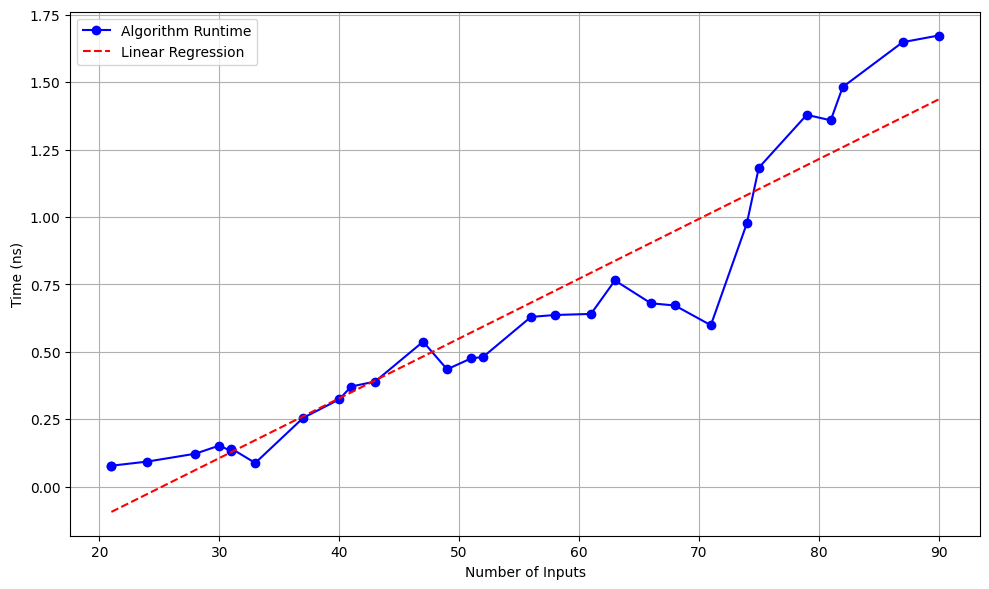
\includegraphics[width=\textwidth]{img/greedy.png}
    \caption{Time taken for the Greedy benchmarks}
    \label{fig:greedy}
\end{figure}

\begin{figure}[h]
    \centering
    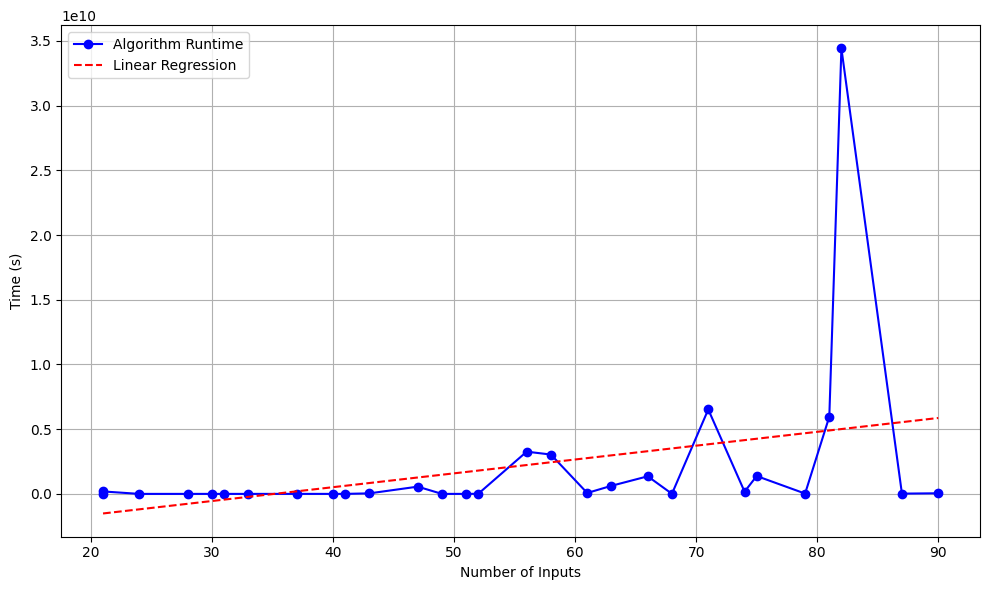
\includegraphics[width=\textwidth]{img/backtracking.png}
    \caption{Time taken for the Backtracking benchmarks}
    \label{fig:backtracking}
\end{figure}

\begin{figure}[h]
    \centering
    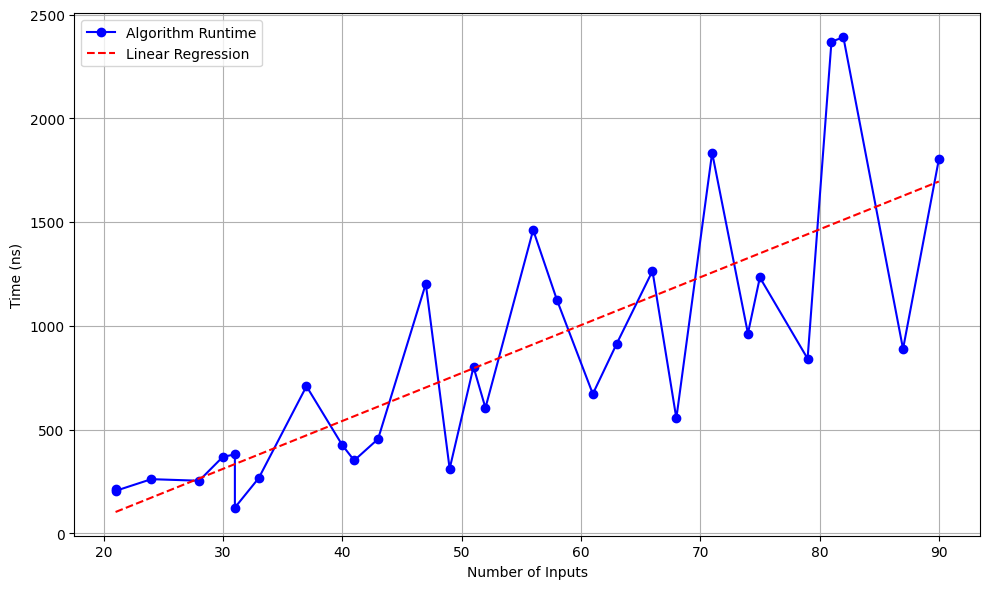
\includegraphics[width=\textwidth]{img/tabulation.png}
    \caption{Time taken for the Tabulation benchmarks}
    \label{fig:tabulation}
\end{figure}
\clearpage

The graphs show the distribution of the performances of the algorithms
based on the number of inputs and the execution time. Every algorithm shows
an ascending trend, meaning that, generally, they take longer to complete
the higher the number of sets of inputs they are given.

Some tests appear to be faster than others that have a smaller input size.
This is predominantly happening becuase the benchmarks were run in a multithreaded
environment, where a lot of context switches were happening and multiple tasks were
running at the same time anyways.

It is easy to say that the tabulation approach is by far the most reliable, albeit
not the fastest. The speed of the greedy approach can be deceiving, suggesting it would be
the best algorithm to solve the problem, but we have to take into consideration the fact
that it does not provide the highest possible profit. Its solution is \textit{almost} correct.
With all of that in mind, if we are not looking for the perfect combination of items, but
for a quick and decent result, the greedy would be the best algorithm. As seen in the second graph,
the backtracking approach is by far the slowest of them all, since it explores every possible combination of items
(time complexity of $\mathcal{O}(2^n)$). Even though it is very slow, it is still better in terms of
the correctness of the result than the greedy algorithm. The only point it actually excels in
is its simplicity of the implementation, as it's a good starting point to understand the problem.

With all of that being said, if we care about achieving a perfect result in a timely manner,
we can conclude that the dynamic programming approach is the best one, and if we want a
solution as fast as possible, although not perfect, the greedy algorithm is the way to go.


\begin{thebibliography}{8}

\bibitem{ref_article1}
\emph{Knapsack problem}, \url{https://en.wikipedia.org/wiki/Knapsack_problem} Accessed at [04/01/2025].

\bibitem{ref_article2}
Kayode Badiru: \emph{KNAPSACK PROBLEMS; METHODS, MODELS AND APPLICATIONS},
\url{https://shareok.org/server/api/core/bitstreams/7bb97e22-4c5d-44b3-b756-74aba3fc1fd7/content} 
Accessed at [05/01/2025]

\bibitem{ref_url1}
LNCS Homepage, \url{http://www.springer.com/lncs}, Accessed at [04/01/2025]

\bibitem{ref_url2}
\emph{A Phase Angle-Modulated Bat Algorithm with Application to Antenna Topology Optimization}
\url{https://www.researchgate.net/publication/349878676_A_Phase_Angle-Modulated_Bat_Algorithm_with_Application_to_Antenna_Topology_Optimization}, Accessed at [04/01/2025]

\bibitem{ref_url3}
Geeks for Geeks, \emph{0/1 Knapsack Problem}, \url{https://www.geeksforgeeks.org/0-1-knapsack-problem-dp-10/}, Accessed at [05/01/2025]

\bibitem{ref_url4}
Cornell University, \emph{ORIE 6300 Mathematical Programming I --- Lecture 25}, \url{https://people.orie.cornell.edu/dpw/orie6300/Lectures/lec25.pdf}, Accessed at [07/01/2025]

\bibitem{ref_url5}
Politehnica Bucharest, \emph{Analiza Algoritmilor Seria CC 2024 --- Capitolul 10 - Probleme NP-Complete}, Accessed at [07/01/2025]

\end{thebibliography}
\end{document}
